% answers.tex —— 2008 年·普通高等学校招生考试·山东卷·文科 · 参考答案与详细解析片段
% 由 tools/generate_projects.py 依来源总账自 2008/2008_数学真题_山东文_试题.md + 2008/2008_数学真题_山东文_解析正文.md + 2008/2008_数学真题_山东文_答案要点.md 生成，勿手改（改源 MD 后重跑）


\begin{gktip}
固定候选 PDF 仅含题面，无答案、解析和评分标准，原卷亦未标注分值；以下为非官方编者独立推导，官方答案字段为空。来源发布者、出版者、版次与官方身份均未核。
\end{gktip}

\begin{answer}
\gksolhead{1}{}

\textbf{题目}：

满足 $M\subseteq\{a_1,a_2,a_3,a_4\}$，且 $M\cap\{a_1,a_2,a_3\}=\{a_1,a_2\}$ 的集合 $M$ 的个数是（　）

（A）$1$

（B）$2$

（C）$3$

（D）$4$

\Needspace{4\baselineskip}
\textbf{解析}

$M$ 必须含 $a_1$，$a_2$，由 $M\cap\{a_1,a_2,a_3\}=\{a_1,a_2\}$ 知 $a_3\notin M$，而 $a_4$ 可含可不含。

故 $M=\{a_1,a_2\}$ 或 $\{a_1,a_2,a_4\}$，共 $2$ 个。

\gkanswer{答案：B。}

\end{answer}
\begin{answer}
\gksolhead{2}{}

\textbf{题目}：

设 $z$ 的共轭复数是 $\bar z$，若 $z+\bar z=4$，$z\cdot\bar z=8$，则 $\dfrac{\bar z}{z}$ 等于（　）

（A）$\mathrm i$

（B）$-\mathrm i$

（C）$\pm1$

（D）$\pm\mathrm i$

\Needspace{4\baselineskip}
\textbf{解析}

由 $z+\bar z=4$ 得 $\operatorname{Re}z=2$；由 $z\bar z=8$ 得 $|z|=2\sqrt2$，故 $z=2\pm2\mathrm i$。

$z=2+2\mathrm i$ 时 $\dfrac{\bar z}z=\dfrac{2-2\mathrm i}{2+2\mathrm i}=-\mathrm i$；$z=2-2\mathrm i$ 时 $\dfrac{\bar z}z=\mathrm i$。

故 $\dfrac{\bar z}z=\pm\mathrm i$。

\gkanswer{答案：D。}

\end{answer}
\begin{answer}
\gksolhead{3}{}

\textbf{题目}：

函数 $y=\ln\cos x$（$-\dfrac{\pi}{2}<x<\dfrac{\pi}{2}$）的图象是（　）
\nopagebreak[4]
\begin{center}% 2008 年山东卷文科第 3 题：函数 y=ln(cos x)（-π/2<x<π/2）图象的四个候选。
% 来源 PDF：gaokaomath-src/普通高考/2008/2008山东文.pdf
% SHA-256：479a9abc0fe5954c5b717d8eb0f649966c1cee3cfabdab00f10cc5834668fd6f
% 原页：2008山东文.pdf 第 1 页（A3 三栏）第 1 栏，书页码 473。
% 布局：四幅小图按 2×2 排布（行距 5.6 单位、列距 4.3 单位），每幅含 x、y 轴、
%   ±π/2 两条虚线渐近线与曲线，(A)～(D) 标在各小图正下方。
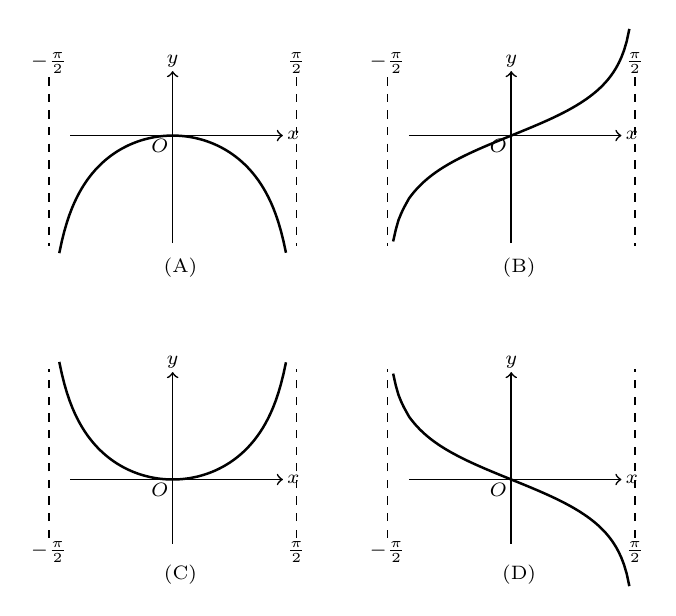
\begin{tikzpicture}[x=1.0cm, y=0.78cm, semithick, font=\scriptsize,
  every node/.style={inner sep=1.2pt}]

  % ---- (A) y = ln(cos x)：偶函数，x=0 处取最大值 0，两端趋于 -inf ----
  \begin{scope}[shift={(0,0)}]
    \draw[->] (-1.30,0) -- (1.40,0) node[right] {$x$};
    \draw[->] (0,-1.75) -- (0,1.05) node[above] {$y$};
    \node[below left] at (0,0) {$O$};
    \draw[dashed] (-1.571,0.95) -- (-1.571,-1.80);
    \draw[dashed] (1.571,0.95) -- (1.571,-1.80);
    \node[above] at (-1.571,0.95) {$-\frac{\pi}{2}$};
    \node[above] at (1.571,0.95) {$\frac{\pi}{2}$};
    \draw[line width=0.9pt, domain=-1.44:1.44, samples=90] plot (\x, {0.95*ln(cos(\x r))});
    \node at (0.10,-2.15) {(A)};
  \end{scope}

  % ---- (B) 递增且过原点 ----
  \begin{scope}[shift={(4.3,0)}]
    \draw[->] (-1.30,0) -- (1.40,0) node[right] {$x$};
    \draw[->] (0,-1.75) -- (0,1.05) node[above] {$y$};
    \node[below left] at (0,0) {$O$};
    \draw[dashed] (-1.571,0.95) -- (-1.571,-1.80);
    \draw[dashed] (1.571,0.95) -- (1.571,-1.80);
    \node[above] at (-1.571,0.95) {$-\frac{\pi}{2}$};
    \node[above] at (1.571,0.95) {$\frac{\pi}{2}$};
    \draw[line width=0.9pt, domain=-1.50:1.50, samples=90]
      plot (\x, {0.52*ln((1+sin(\x r))/cos(\x r))});
    \node at (0.10,-2.15) {(B)};
  \end{scope}

  % ---- (C) y = -ln(cos x) ----
  \begin{scope}[shift={(0,-5.6)}]
    \draw[->] (-1.30,0) -- (1.40,0) node[right] {$x$};
    \draw[->] (0,-1.05) -- (0,1.75) node[above] {$y$};
    \node[below left] at (0,0) {$O$};
    \draw[dashed] (-1.571,-0.95) -- (-1.571,1.80);
    \draw[dashed] (1.571,-0.95) -- (1.571,1.80);
    \node[below] at (-1.571,-0.95) {$-\frac{\pi}{2}$};
    \node[below] at (1.571,-0.95) {$\frac{\pi}{2}$};
    \draw[line width=0.9pt, domain=-1.44:1.44, samples=90] plot (\x, {-0.95*ln(cos(\x r))});
    \node at (0.10,-1.55) {(C)};
  \end{scope}

  % ---- (D) 递减且过原点 ----
  \begin{scope}[shift={(4.3,-5.6)}]
    \draw[->] (-1.30,0) -- (1.40,0) node[right] {$x$};
    \draw[->] (0,-1.05) -- (0,1.75) node[above] {$y$};
    \node[below left] at (0,0) {$O$};
    \draw[dashed] (-1.571,-0.95) -- (-1.571,1.80);
    \draw[dashed] (1.571,-0.95) -- (1.571,1.80);
    \node[below] at (-1.571,-0.95) {$-\frac{\pi}{2}$};
    \node[below] at (1.571,-0.95) {$\frac{\pi}{2}$};
    \draw[line width=0.9pt, domain=-1.50:1.50, samples=90]
      plot (\x, {-0.52*ln((1+sin(\x r))/cos(\x r))});
    \node at (0.10,-1.55) {(D)};
  \end{scope}
\end{tikzpicture}
\end{center}
\nopagebreak[4]
\Needspace{4\baselineskip}
\textbf{解析}

\Needspace{5\baselineskip}
$f(x)=\ln\cos x$ 是偶函数，$f(0)=0$，且

\nopagebreak[4]
\[f''(x)=-\sec^2x<0,\]

故图象在 $\left(-\dfrac{\pi}{2},\dfrac{\pi}{2}\right)$ 上为上凸（“$\cap$”形），在 $x=0$ 处取最大值 $0$；当 $x\to\pm\dfrac{\pi}{2}$ 时 $\cos x\to0^+$，$f(x)\to-\infty$，即 $x=\pm\dfrac{\pi}{2}$ 为两条竖直渐近线。

与四个候选图对照，只有 (A) 符合。

\gkanswer{答案：A。}

\end{answer}
\begin{answer}
\gksolhead{4}{}

\textbf{题目}：

给出命题：若函数 $y=f(x)$ 是幂函数，则函数 $y=f(x)$ 的图象不过第四象限。在它的逆命题、否命题、逆否命题三个命题中，真命题的个数是（　）

（A）$3$

（B）$2$

（C）$1$

（D）$0$

\Needspace{4\baselineskip}
\textbf{解析}

原命题：$p$（是幂函数）$\Rightarrow$ $q$（图象不过第四象限），为真。

逆命题 $q\Rightarrow p$：$y=\mathrm e^x$ 的图象不过第四象限，但它不是幂函数，假。

否命题 $\neg p\Rightarrow\neg q$：与逆命题等价，假。

逆否命题 $\neg q\Rightarrow\neg p$：与原命题等价，为真。

故真命题只有 $1$ 个。

\gkanswer{答案：C。}

\end{answer}
\begin{answer}
\gksolhead{5}{}

\textbf{题目}：

设函数 $f(x)=\begin{cases}1-x^2,&x\leqslant1,\\ x^2+x-2,&x>1,\end{cases}$ 则 $f\left(\dfrac1{f(2)}\right)$ 的值为（　）

（A）$\dfrac{15}{16}$

（B）$-\dfrac{27}{16}$

（C）$\dfrac89$

（D）$18$

\Needspace{4\baselineskip}
\textbf{解析}

\Needspace{5\baselineskip}
$2>1$，故 $f(2)=2^2+2-2=4$，于是 $\dfrac1{f(2)}=\dfrac14\leqslant1$，

\nopagebreak[4]
\[f\left(\frac14\right)=1-\left(\frac14\right)^2=\frac{15}{16}.\]

\gkanswer{答案：A。}

\end{answer}
\begin{answer}
\gksolhead{6}{}

\textbf{题目}：

如图是一个几何体的三视图，根据图中数据，可得该几何体的表面积是（　）
\nopagebreak[4]
\begin{center}% 2008 年山东卷文科第 6 题：几何体的三视图（圆柱上放一个等径的球）。
% 来源 PDF：gaokaomath-src/普通高考/2008/2008山东文.pdf
% SHA-256：479a9abc0fe5954c5b717d8eb0f649966c1cee3cfabdab00f10cc5834668fd6f
% 原页：2008山东文.pdf 第 1 页（A3 三栏）第 1 栏，书页码 473。
% 重绘依据：正视图为宽 2、高 3 的矩形上切一个直径 2 的圆（球与圆柱同径，相切于上底），
%   侧视图同形，俯视图为直径 2 的圆；尺寸 2、3、2 按原图标注。
\begin{tikzpicture}[semithick, font=\small, every node/.style={inner sep=1.2pt}]
  % 正（主）视图
  \begin{scope}[shift={(0,0)}]
    \draw (0,0) rectangle (2,3);
    \draw (1,4) circle (1);
    \draw[<->] (2.35,0) -- (2.35,3) node[midway,right] {$3$};
    \draw[<->] (0,-0.35) -- (2,-0.35) node[midway,below] {$2$};
    \draw[<->] (2.35,3) -- (2.35,5) node[midway,right] {$2$};
    \node at (1,-1.15) {正（主）视图};
  \end{scope}
  % 侧（左）视图
  \begin{scope}[shift={(5.2,0)}]
    \draw (0,0) rectangle (2,3);
    \draw (1,4) circle (1);
    \draw[<->] (0,-0.35) -- (2,-0.35) node[midway,below] {$2$};
    \node at (1,-1.15) {侧（左）视图};
  \end{scope}
  % 俯视图
  \begin{scope}[shift={(2.6,-4.4)}]
    \draw (0,0) circle (1);
    \draw[<->] (0,-1.4) -- (2,-1.4) node[midway,below] {$2$};
    \node at (1,-2.15) {俯视图};
  \end{scope}
\end{tikzpicture}
\end{center}
\nopagebreak[4]
（A）$9\pi$

（B）$10\pi$

（C）$11\pi$

（D）$12\pi$

\Needspace{4\baselineskip}
\textbf{解析}

由三视图，该几何体是底面半径为 $1$、高为 $3$ 的圆柱，上面放一个半径为 $1$ 的球。

\Needspace{5\baselineskip}
圆柱侧面积 $2\pi\cdot1\cdot3=6\pi$，圆柱底面积 $\pi\cdot1^2=\pi$，球面积 $4\pi\cdot1^2=4\pi$；圆柱上底面被球遮住，不计。

\nopagebreak[4]
\[S=6\pi+\pi+4\pi=11\pi.\]

\gkanswer{答案：C。}

\end{answer}
\begin{answer}
\gksolhead{7}{}

\textbf{题目}：

不等式 $\dfrac{x+5}{(x-1)^2}\geqslant2$ 的解集是（　）

（A）$\left[-3,\frac12\right]$

（B）$\left[-\frac12,3\right]$

（C）$\left[\frac12,1\right)\cup(1,3]$

（D）$\left[-\frac12,1\right)\cup(1,3]$

\Needspace{4\baselineskip}
\textbf{解析}

\Needspace{5\baselineskip}
因 $(x-1)^2>0$（$x\neq1$），原不等式等价于

\nopagebreak[4]
\[x+5\geqslant2(x-1)^2\ \Longleftrightarrow\ 2x^2-5x-3\leqslant0\ \Longleftrightarrow\ (2x+1)(x-3)\leqslant0,\]

即 $-\dfrac12\leqslant x\leqslant3$，又 $x\neq1$，故解集为 $\left[-\dfrac12,1\right)\cup(1,3]$。

\gkanswer{答案：D。}

\end{answer}
\begin{answer}
\gksolhead{8}{}

\textbf{题目}：

已知 $a$，$b$，$c$ 为 $\triangle ABC$ 的三个内角 $A$，$B$，$C$ 的对边，向量 $\boldsymbol m=(\sqrt3,-1)$，$\boldsymbol n=(\cos A,\sin A)$。若 $\boldsymbol m\perp\boldsymbol n$，且 $a\cos B+b\cos A=c\sin C$，则角 $A$，$B$ 的大小分别为（　）

（A）$\dfrac{\pi}{6}$，$\dfrac{\pi}{3}$

（B）$\dfrac{2\pi}{3}$，$\dfrac{\pi}{6}$

（C）$\dfrac{\pi}{3}$，$\dfrac{\pi}{6}$

（D）$\dfrac{\pi}{3}$，$\dfrac{\pi}{3}$

\Needspace{4\baselineskip}
\textbf{解析}

\Needspace{5\baselineskip}
由 $\boldsymbol m\perp\boldsymbol n$ 得

\nopagebreak[4]
\[\sqrt3\cos A-\sin A=0\ \Longrightarrow\ \tan A=\sqrt3,\]

$A\in(0,\pi)$，故 $A=\dfrac{\pi}3$。

\Needspace{5\baselineskip}
由正弦定理，$a\cos B+b\cos A=2R(\sin A\cos B+\sin B\cos A)=2R\sin(A+B)=2R\sin C$，而 $c\sin C=2R\sin^2C$，故

\nopagebreak[4]
\[\sin C=\sin^2C\ \Longrightarrow\ \sin C=1,\]

即 $C=\dfrac{\pi}2$，从而 $B=\pi-\dfrac{\pi}3-\dfrac{\pi}2=\dfrac{\pi}6$。

\gkanswer{答案：C。}

\end{answer}
\begin{answer}
\gksolhead{9}{}

\textbf{题目}：

从某项综合能力测试中抽取 $100$ 人的成绩，统计如表，则这 $100$ 人成绩的标准差为（　）

\begin{center}
\begin{tabular}{llllll}
\toprule
分数 & $5$ & $4$ & $3$ & $2$ & $1$ \\
\midrule
人数 & $20$ & $10$ & $30$ & $30$ & $10$ \\
\bottomrule
\end{tabular}
\end{center}

（A）$\sqrt3$

（B）$\dfrac{2\sqrt{10}}5$

（C）$3$

（D）$\dfrac85$

\Needspace{4\baselineskip}
\textbf{解析}

\Needspace{5\baselineskip}
平均分

\nopagebreak[4]
\[\bar x=\frac{5\times20+4\times10+3\times30+2\times30+1\times10}{100}=3.\]

\Needspace{5\baselineskip}
方差

\nopagebreak[4]
\[s^2=\frac{20(5-3)^2+10(4-3)^2+30(3-3)^2+30(2-3)^2+10(1-3)^2}{100}=\frac{160}{100}=\frac85,\]

故标准差 $s=\sqrt{\dfrac85}=\dfrac{2\sqrt{10}}5$。

\gkanswer{答案：B。}

\end{answer}
\begin{answer}
\gksolhead{10}{}

\textbf{题目}：

已知 $\cos\left(\alpha-\dfrac{\pi}{6}\right)+\sin\alpha=\dfrac45\sqrt3$，则 $\sin\left(\alpha+\dfrac{7\pi}{6}\right)$ 的值是（　）

（A）$-\dfrac{2\sqrt3}5$

（B）$\dfrac{2\sqrt3}5$

（C）$-\dfrac45$

（D）$\dfrac45$

\Needspace{4\baselineskip}
\textbf{解析}

\Needspace{5\baselineskip}
计算如下：

\nopagebreak[4]
\[\cos\left(\alpha-\frac{\pi}6\right)+\sin\alpha=\frac{\sqrt3}2\cos\alpha+\frac32\sin\alpha=\frac{4\sqrt3}5,\]

两边乘 $\dfrac2{\sqrt3}$ 得 $\cos\alpha+\sqrt3\sin\alpha=\dfrac85$。

\Needspace{5\baselineskip}
于是

\nopagebreak[4]
\[\sin\left(\alpha+\frac{7\pi}6\right)=-\sin\left(\alpha+\frac{\pi}6\right)=-\frac12\left(\sqrt3\sin\alpha+\cos\alpha\right)=-\frac45.\]

\gkanswer{答案：C。}

\end{answer}
\begin{answer}
\gksolhead{11}{}

\textbf{题目}：

若圆 $C$ 的半径为 $1$，圆心在第一象限，且与直线 $4x-3y=0$ 和 $x$ 轴相切，则该圆的标准方程是（　）

（A）$(x-3)^2+\left(y-\dfrac73\right)^2=1$

（B）$(x-2)^2+(y-1)^2=1$

（C）$(x-1)^2+(y-3)^2=1$

（D）$\left(x-\dfrac32\right)^2+(y-1)^2=1$

\Needspace{4\baselineskip}
\textbf{解析}

圆与 $x$ 轴相切且半径为 $1$、圆心在第一象限，故圆心为 $(a,1)$（$a>0$）。

\Needspace{5\baselineskip}
圆心到直线 $4x-3y=0$ 的距离等于半径：

\nopagebreak[4]
\[\frac{|4a-3|}5=1\ \Longrightarrow\ 4a-3=\pm5,\]

\Needspace{5\baselineskip}
得 $a=2$（$a=-\dfrac12$ 舍去）。故圆为

\nopagebreak[4]
\[(x-2)^2+(y-1)^2=1.\]

\gkanswer{答案：B。}

\end{answer}
\begin{answer}
\gksolhead{12}{}

\textbf{题目}：

已知函数 $f(x)=\log_a(2^x+b-1)$（$a>0$，$a\neq1$）的图象如图所示，则 $a$，$b$ 满足的关系是（　）
\nopagebreak[4]
\begin{center}% 2008 年山东卷文科第 12 题：f(x)=log_a(2^x+b-1) 的图象，与 y 轴交点高于 y=-1。
% 来源 PDF：gaokaomath-src/普通高考/2008/2008山东文.pdf
% SHA-256：479a9abc0fe5954c5b717d8eb0f649966c1cee3cfabdab00f10cc5834668fd6f
% 原页：2008山东文.pdf 第 1 页（A3 三栏）第 2 栏，书页码 473。
\begin{tikzpicture}[x=1.7cm, y=1.05cm, semithick, font=\small,
  every node/.style={inner sep=1.2pt}]
  \draw[->,>=stealth] (-1.5,0) -- (1.9,0) node[right] {$x$};
  \draw[->,>=stealth] (0,-1.55) -- (0,1.5) node[above] {$y$};
  \node[below left] at (0,0) {$O$};
  \draw (0,-1) -- (-0.05,-1);
  \node[left] at (-0.05,-1) {$-1$};
  % 曲线：单调递增，与 y 轴交于 -0.45（高于 -1），与 x 轴交于正半轴
  \draw[line width=0.9pt] (-1.15,-1.25)
    .. controls (-0.60,-0.95) and (-0.28,-0.62) .. (0,-0.45)
    .. controls (0.45,-0.17) and (1.00,0.28) .. (1.72,0.80);
\end{tikzpicture}
\end{center}
\nopagebreak[4]
（A）$0<a^{-1}<b<1$

（B）$0<b<a^{-1}<1$

（C）$0<b^{-1}<a<-1$

（D）$0<a^{-1}<b^{-1}<1$

\Needspace{4\baselineskip}
\textbf{解析}

\Needspace{5\baselineskip}
图象与 $y$ 轴的交点在 $y=-1$ 的上方且在 $x$ 轴下方：

\nopagebreak[4]
\[-1<\log_ab<0.\]

图象单调递增，故 $a>1$，于是 $\log_ab<0$ 给出 $0<b<1$；而 $-1<\log_ab$ 即 $\log_a\dfrac1a<\log_ab$，得 $b>a^{-1}$。

故 $0<a^{-1}<b<1$。

\gkanswer{答案：A。}

\end{answer}
\begin{answer}
\gksolhead{13}{}

\textbf{题目}：

已知圆 $C$：$x^2+y^2-6x-4y+8=0$。以圆 $C$ 与坐标轴的交点分别作为双曲线的一个焦点和顶点，则适合上述条件的双曲线的标准方程为\gkblank{}。

\Needspace{4\baselineskip}
\textbf{解析}

\Needspace{5\baselineskip}
计算如下：

\nopagebreak[4]
\[x^2+y^2-6x-4y+8=0\ \Longleftrightarrow\ (x-3)^2+(y-2)^2=5.\]

与 $x$ 轴（$y=0$）交于 $x^2-6x+8=0$，即 $x=2$，$4$，得 $(2,0)$，$(4,0)$；与 $y$ 轴无交点（$y^2-4y+8=0$ 判别式为负）。

\Needspace{5\baselineskip}
以 $(4,0)$ 为焦点、$(2,0)$ 为顶点，则 $c=4$，$a=2$，

\nopagebreak[4]
\[b^2=c^2-a^2=12,\]

故双曲线为 $\dfrac{x^2}4-\dfrac{y^2}{12}=1$。

\gkanswer{答案：$\dfrac{x^2}4-\dfrac{y^2}{12}=1$。}

\end{answer}
\begin{answer}
\gksolhead{14}{}

\textbf{题目}：

执行下面的程序框图，若 $p=0.8$，则输出的 $n=$\gkblank{}。
\nopagebreak[4]
\begin{center}% 2008 年山东卷文科第 14 题：程序框图。
% 来源 PDF：gaokaomath-src/普通高考/2008/2008山东文.pdf
% SHA-256：479a9abc0fe5954c5b717d8eb0f649966c1cee3cfabdab00f10cc5834668fd6f
% 原页：2008山东文.pdf 第 1 页（A3 三栏）第 3 栏，书页码 473。
\begin{tikzpicture}[>=stealth, semithick, font=\small,
  every node/.style={inner sep=2pt},
  box/.style={draw, minimum width=2.4cm, minimum height=0.7cm},
  term/.style={draw, rounded corners=6pt, minimum width=1.6cm, minimum height=0.6cm},
  io/.style={draw, trapezium, trapezium left angle=110, trapezium right angle=70,
             minimum width=2.0cm, minimum height=0.7cm},
  dec/.style={draw, diamond, aspect=1.7, minimum width=2.3cm, minimum height=1.0cm}]

  \node[term] (s) at (0,0) {开始};
  \node[io]   (in) at (0,-1.3) {输入 $p$};
  \node[box]  (ini) at (0,-2.6) {$n=1$，$S=0$};
  \node[dec]  (jud) at (0,-4.1) {$S<p$?};
  \node[box]  (acc) at (0,-5.5) {$S=S+\dfrac1{2^n}$};
  \node[box]  (inc) at (0,-6.7) {$n=n+1$};
  \node[io]   (out) at (3.6,-4.1) {输出 $n$};
  \node[term] (end) at (3.6,-5.3) {结束};

  \draw[->] (s) -- (in);
  \draw[->] (in) -- (ini);
  \draw[->] (ini) -- (jud);
  \draw[->] (jud) -- node[right] {是} (acc);
  \draw[->] (acc) -- (inc);
  \draw[->] (jud) -- node[above] {否} (out);
  \draw[->] (out) -- (end);

  % 回路上行：从 n=n+1 的左侧回到判定框上方
  \draw[->] (inc.west) -- (-2.6,-6.7) -- (-2.6,-2.6) -- (ini.west);
\end{tikzpicture}
\end{center}
\nopagebreak[4]
\Needspace{4\baselineskip}
\textbf{解析}

依次执行：$n=1$，$S=0$。

$S=0<0.8$，$S=0+\dfrac12=\dfrac12$，$n=2$；

$S=\dfrac12<0.8$，$S=\dfrac12+\dfrac14=\dfrac34$，$n=3$；

$S=\dfrac34<0.8$，$S=\dfrac34+\dfrac18=\dfrac78$，$n=4$；

$S=\dfrac78\geqslant0.8$，跳出循环，输出 $n=4$。

\gkanswer{答案：$4$。}

\end{answer}
\begin{answer}
\gksolhead{15}{}

\textbf{题目}：

已知 $f(3^x)=4x\log_23+233$，则 $f(2)+f(4)+f(8)+\cdots+f(2^8)$ 的值等于\gkblank{}。

\Needspace{4\baselineskip}
\textbf{解析}

\Needspace{5\baselineskip}
令 $t=3^x$，则 $x=\log_3t$，于是

\nopagebreak[4]
\[f(t)=4\log_3t\cdot\log_23+233=4\log_2t+233.\]

\Needspace{5\baselineskip}
故

\nopagebreak[4]
\[\sum_{k=1}^{8}f(2^k)=\sum_{k=1}^{8}\left(4k+233\right)=4\times36+8\times233=144+1864=2008.\]

\gkanswer{答案：$2008$。}

\end{answer}
\begin{answer}
\gksolhead{16}{}

\textbf{题目}：

设 $x$，$y$ 满足约束条件 $\begin{cases}x-y+2\geqslant0,\\ 5x-y-10\leqslant0,\\ x\geqslant0,\\ y\geqslant0,\end{cases}$ 则 $z=2x+y$ 的最大值为\gkblank{}。

\Needspace{4\baselineskip}
\textbf{解析}

\Needspace{5\baselineskip}
可行域顶点为 $(0,0)$，$(0,2)$，$(2,0)$，以及 $x-y+2=0$ 与 $5x-y-10=0$ 的交点 $(3,5)$。

\nopagebreak[4]
\[z=2x+y\quad\Rightarrow\quad 0,\ 2,\ 4,\ 11,\]

故最大值为 $11$。

\gkanswer{答案：$11$。}

\end{answer}
\begin{answer}
\gksolhead{17}{}

\textbf{题目}：

已知函数 $f(x)=\sqrt3\sin(\omega x+\varphi)-\cos(\omega x+\varphi)$（$0<\varphi<\pi$，$\omega>0$）为偶函数，且函数 $y=f(x)$ 图象的两相邻对称轴间的距离为 $\dfrac{\pi}{2}$。

（1）求 $f\left(\dfrac{\pi}{8}\right)$ 的值；

（2）将函数 $y=f(x)$ 的图象向右平移 $\dfrac{\pi}{6}$ 个单位后，得到函数 $y=g(x)$ 的图象，求 $g(x)$ 的单调递减区间。

\Needspace{4\baselineskip}
\textbf{解析}

\Needspace{5\baselineskip}
（1）

\nopagebreak[4]
\[f(x)=2\sin\left(\omega x+\varphi-\frac{\pi}6\right).\]

\Needspace{5\baselineskip}
$f$ 为偶函数，故其图象关于 $y$ 轴对称，$\omega x+\varphi-\dfrac{\pi}6$ 的初相须为 $\dfrac{\pi}2+k\pi$：

\nopagebreak[4]
\[\varphi=\frac{2\pi}3+k\pi,\]

由 $0<\varphi<\pi$ 得 $\varphi=\dfrac{2\pi}3$，于是 $f(x)=2\sin\left(\omega x+\dfrac{\pi}2\right)=2\cos\omega x$。

\Needspace{5\baselineskip}
相邻对称轴间的距离为半个周期，故 $\dfrac{T}2=\dfrac{\pi}2$，$T=\pi$，$\omega=2$。

\nopagebreak[4]
\[f\left(\frac{\pi}8\right)=2\cos\frac{\pi}4=\sqrt2.\]

\Needspace{5\baselineskip}
（2）向右平移 $\dfrac{\pi}6$ 得

\nopagebreak[4]
\[g(x)=f\left(x-\frac{\pi}6\right)=2\cos\left(2x-\frac{\pi}3\right).\]

\Needspace{5\baselineskip}
$g$ 递减当且仅当

\nopagebreak[4]
\[2x-\frac{\pi}3\in\left[2k\pi,\ \pi+2k\pi\right],\]

\Needspace{5\baselineskip}
即

\nopagebreak[4]
\[x\in\left[\frac{\pi}6+k\pi,\ \frac{2\pi}3+k\pi\right]\quad(k\in\mathbf Z).\]

\gkanswer{答案：（1）$\sqrt2$；（2）$\left[\dfrac{\pi}6+k\pi,\dfrac{2\pi}3+k\pi\right]$（$k\in\mathbf Z$）。}

\end{answer}
\begin{answer}
\gksolhead{18}{}

\textbf{题目}：

现有 $8$ 名奥运会志愿者，其中志愿者 $A_1$，$A_2$，$A_3$ 通晓日语，$B_1$，$B_2$，$B_3$ 通晓俄语，$C_1$，$C_2$ 通晓韩语。从中选出通晓日语、俄语和韩语的志愿者各 $1$ 名，组成一个小组。

（1）求 $A_1$ 被选中的概率；

（2）求 $B_1$ 和 $C_1$ 不全被选中的概率。

\Needspace{4\baselineskip}
\textbf{解析}

选法总数为 $3\times3\times2=18$（日语、俄语、韩语各选 $1$ 名）。

\Needspace{5\baselineskip}
（1）$A_1$ 被选中时，其余两类各选 $1$ 名，共 $1\times3\times2=6$ 种：

\nopagebreak[4]
\[P=\frac6{18}=\frac13.\]

\Needspace{5\baselineskip}
（2）$B_1$ 与 $C_1$ 同时被选中：日语任选 $1$ 名，共 $3$ 种，故

\nopagebreak[4]
\[P(B_1,C_1\text{ \text{同时被选中}})=\frac3{18}=\frac16,\]

\Needspace{5\baselineskip}
所求为

\nopagebreak[4]
\[1-\frac16=\frac56.\]

\gkanswer{答案：（1）$\dfrac13$；（2）$\dfrac56$。}

\end{answer}
\begin{answer}
\gksolhead{19}{}

\textbf{题目}：

如图，在四棱锥 $P-ABCD$ 中，平面 $PAD\perp$ 平面 $ABCD$，$AB\parallel DC$，$\triangle PAD$ 是等边三角形，已知 $BD=2AD=8$，$AB=2DC=4\sqrt5$。

（1）设 $M$ 是 $PC$ 上的一点，证明：平面 $MBD\perp$ 平面 $PAD$；

（2）求四棱锥 $P-ABCD$ 的体积。
\nopagebreak[4]
\begin{center}% 2008 年山东卷文科第 19 题：四棱锥 P-ABCD，平面 PAD⊥平面 ABCD，AB∥DC，
%   △PAD 为等边三角形，BD=2AD=8，AB=2DC=4√5，M 为 PC 上一点。
% 来源 PDF：gaokaomath-src/普通高考/2008/2008山东文.pdf
% SHA-256：479a9abc0fe5954c5b717d8eb0f649966c1cee3cfabdab00f10cc5834668fd6f
% 原页：2008山东文.pdf 第 2 页（A3 三栏）第 1 栏，书页码 474。
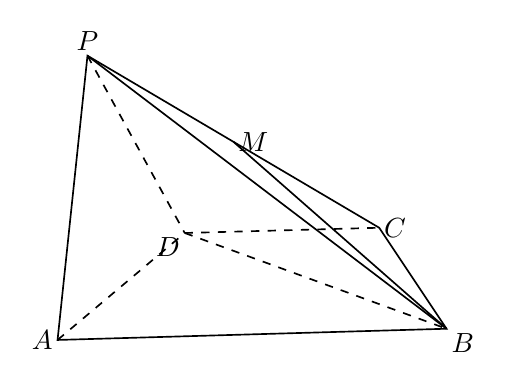
\begin{tikzpicture}[scale=0.95, semithick,
  every node/.style={inner sep=1.5pt}]
  \coordinate (A) at (0.70,0.60);
  \coordinate (B) at (5.90,0.75);
  \coordinate (C) at (5.00,2.10);
  \coordinate (D) at (2.40,2.03);
  \coordinate (P) at (1.10,4.40);
  \coordinate (M) at (3.05,3.25);

  % 可见棱
  \draw (A) -- (B) -- (C) -- (P) -- cycle;
  \draw (P) -- (B);
  \draw (M) -- (B);

  % 被遮挡的棱
  \draw[dashed] (P) -- (D);
  \draw[dashed] (A) -- (D) -- (C);
  \draw[dashed] (D) -- (B);

  \node[above] at (P) {$P$};
  \node[left] at (A) {$A$};
  \node[below right] at (B) {$B$};
  \node[right] at (C) {$C$};
  \node[below left] at (D) {$D$};
  \node[right] at (M) {$M$};
\end{tikzpicture}
\end{center}
\nopagebreak[4]
\Needspace{4\baselineskip}
\textbf{解析}

\Needspace{5\baselineskip}
（1）在 $\triangle ABD$ 中，$AD=4$，$BD=8$，$AB=4\sqrt5$，有

\nopagebreak[4]
\[AD^2+BD^2=16+64=80=AB^2,\]

故 $AD\perp BD$。

\Needspace{5\baselineskip}
平面 $PAD\perp$ 平面 $ABCD$，交线为 $AD$，而 $BD\subset$ 平面 $ABCD$ 且 $BD\perp AD$，故

\nopagebreak[4]
\[BD\perp\text{\text{平面} }PAD.\]

又 $BD\subset$ 平面 $MBD$，所以平面 $MBD\perp$ 平面 $PAD$。

（2）四边形 $ABCD$ 为梯形：$AB\parallel DC$，$AB=4\sqrt5$，$DC=2\sqrt5$。

\Needspace{5\baselineskip}
点 $D$ 到直线 $AB$ 的距离就是梯形的高。取 $D$ 为原点，$DA$ 为 $x$ 轴正方向，$DB$ 为 $y$ 轴正方向，则 $A(4,0)$，$B(0,8)$，直线 $AB$：$2x+y=8$，故

\nopagebreak[4]
\[h=\frac{|0+0-8|}{\sqrt5}=\frac8{\sqrt5}.\]

\Needspace{5\baselineskip}
梯形面积

\nopagebreak[4]
\[S=\frac12\left(4\sqrt5+2\sqrt5\right)\cdot\frac8{\sqrt5}=24.\]

\Needspace{5\baselineskip}
$\triangle PAD$ 为边长 $4$ 的等边三角形，其高为 $2\sqrt3$；因平面 $PAD\perp$ 底面且交线为 $AD$，该高即为四棱锥的高。

\nopagebreak[4]
\[V=\frac13\times24\times2\sqrt3=16\sqrt3.\]

\gkanswer{答案：（1）证明见解析；（2）$16\sqrt3$。}

\end{answer}
\begin{answer}
\gksolhead{20}{}

\textbf{题目}：

\Needspace{5\baselineskip}
将数列 $\{a_n\}$ 中的所有项按每一行比上一行多一项的规则排成如下数表：

\nopagebreak[4]
\[\begin{array}{ccccccc}
a_1&&&&&&\\
a_2&a_3&&&&&\\
a_4&a_5&a_6&&&&\\
a_7&a_8&a_9&a_{10}&&&\\
\cdots&\cdots&\cdots&\cdots&\cdots&\cdots&\cdots
\end{array}\]

记表中的第一列数 $a_1$，$a_2$，$a_4$，$a_7$，$\cdots$ 构成的数列为 $\{b_n\}$，$b_1=a_1=1$。$S_n$ 为数列 $\{b_n\}$ 的前 $n$ 项和，且满足 $\dfrac{2b_n}{b_nS_n-S_n^2}=1$（$n\geqslant2$）。

（1）证明数列 $\left\{\dfrac1{S_n}\right\}$ 成等差数列，并求数列 $\{b_n\}$ 的通项公式；

（2）上表中，若从第三行起，每一行中的数按从左到右的顺序均构成等比数列，且公比为同一个正数。当 $a_{81}=-\dfrac4{91}$ 时，求上表中第 $k$（$k\geqslant3$）行所有项的和。

\Needspace{4\baselineskip}
\textbf{解析}

\Needspace{5\baselineskip}
（1）由 $b_n=S_n-S_{n-1}$ 与 $\dfrac{2b_n}{b_nS_n-S_n^2}=1$ 得

\nopagebreak[4]
\[2b_n=b_nS_n-S_n^2=(S_n-S_{n-1})S_n-S_n^2=-S_nS_{n-1}.\]

\Needspace{5\baselineskip}
两边除以 $S_nS_{n-1}$：

\nopagebreak[4]
\[\frac2{S_{n-1}}-\frac2{S_n}=-1\ \Longrightarrow\ \frac1{S_n}-\frac1{S_{n-1}}=\frac12\quad(n\geqslant2).\]

\Needspace{5\baselineskip}
故 $\left\{\dfrac1{S_n}\right\}$ 是首项 $\dfrac1{S_1}=\dfrac1{b_1}=1$、公差 $\dfrac12$ 的等差数列，

\nopagebreak[4]
\[\frac1{S_n}=1+\frac{n-1}2=\frac{n+1}2,\qquad S_n=\frac2{n+1}.\]

\Needspace{5\baselineskip}
于是

\nopagebreak[4]
\[b_1=1,\qquad b_n=S_n-S_{n-1}=\frac2{n+1}-\frac2n=-\frac{2}{n(n+1)}\ (n\geqslant2).\]

\Needspace{5\baselineskip}
（2）第 $k$ 行有 $k$ 项，其首项为 $b_k$（第一列），末项为 $a_{N_k}$，其中

\nopagebreak[4]
\[N_k=1+\frac{k(k-1)}2.\]

\Needspace{5\baselineskip}
当 $k=13$ 时 $N_{13}=79$，故 $a_{81}$ 是第 $13$ 行的第 $3$ 项。设公比为 $q>0$，则

\nopagebreak[4]
\[a_{81}=b_{13}q^2.\]

\Needspace{5\baselineskip}
由 $b_{13}=-\dfrac2{13\times14}=-\dfrac1{91}$ 得

\nopagebreak[4]
\[-\frac{q^2}{91}=-\frac4{91}\ \Longrightarrow\ q^2=4,\qquad q=2.\]

\Needspace{5\baselineskip}
故第 $k$ 行各项之和为

\nopagebreak[4]
\[S=b_k\left(1+q+\cdots+q^{k-1}\right)=-\frac{2}{k(k+1)}\left(2^k-1\right)=-\frac{2(2^k-1)}{k(k+1)}.\]

\gkanswer{答案：（1）$\left\{\dfrac1{S_n}\right\}$ 是公差 $\dfrac12$ 的等差数列，$b_1=1$，$b_n=-\dfrac{2}{n(n+1)}$（$n\geqslant2$）；（2）$-\dfrac{2(2^k-1)}{k(k+1)}$。}

\end{answer}
\begin{answer}
\gksolhead{21}{}

\textbf{题目}：

设函数 $f(x)=x^2\mathrm e^{x-1}+ax^3+bx^2$，已知 $x=-2$ 和 $x=1$ 为 $f(x)$ 的极值点。

（1）求 $a$ 和 $b$ 的值；

（2）讨论 $f(x)$ 的单调性；

（3）设 $g(x)=\dfrac23x^3-x^2$，试比较 $f(x)$ 与 $g(x)$ 的大小。

\Needspace{4\baselineskip}
\textbf{解析}

\Needspace{5\baselineskip}
（1）

\nopagebreak[4]
\[f'(x)=\mathrm e^{x-1}\left(x^2+2x\right)+3ax^2+2bx.\]

由 $f'(1)=0$ 得 $3+3a+2b=0$；由 $f'(-2)=0$ 得 $\mathrm e^{-3}(4-4)+12a-4b=0$，即 $b=3a$。

\Needspace{5\baselineskip}
代入得 $3+3a+6a=0$，故

\nopagebreak[4]
\[a=-\frac13,\qquad b=-1.\]

\Needspace{5\baselineskip}
（2）此时

\nopagebreak[4]
\[f'(x)=\mathrm e^{x-1}\left(x^2+2x\right)-x^2-2x=(x+2)x\left(\mathrm e^{x-1}-1\right).\]

符号：$x<-2$ 时三个因式均为负，$f'<0$；$-2<x<0$ 时 $x+2>0$、$x<0$、$\mathrm e^{x-1}-1<0$，$f'>0$；$0<x<1$ 时 $f'<0$；$x>1$ 时 $f'>0$。

故 $f$ 在 $(-\infty,-2)$ 与 $(0,1)$ 上递减，在 $(-2,0)$ 与 $(1,+\infty)$ 上递增。

\Needspace{5\baselineskip}
（3）

\nopagebreak[4]
\[f(x)-g(x)=x^2\mathrm e^{x-1}-\frac13x^3-x^2-\frac23x^3+x^2=x^2\left(\mathrm e^{x-1}-x\right).\]

记 $h(x)=\mathrm e^{x-1}-x$，则 $h'(x)=\mathrm e^{x-1}-1$，$h$ 在 $x=1$ 处取最小值 $h(1)=0$，故 $h(x)\geqslant0$。

于是 $f(x)-g(x)=x^2h(x)\geqslant0$，即 $f(x)\geqslant g(x)$，等号当且仅当 $x=0$ 或 $x=1$。

\gkanswer{答案：（1）$a=-\dfrac13$，$b=-1$；（2）减区间 $(-\infty,-2)$、$(0,1)$，增区间 $(-2,0)$、$(1,+\infty)$；（3）$f(x)\geqslant g(x)$，等号仅在 $x=0$ 或 $x=1$ 处成立。}

\end{answer}
\begin{answer}
\gksolhead{22}{}

\textbf{题目}：

已知曲线 $C_1$：$\dfrac{|x|}a+\dfrac{|y|}b=1$（$a>b>0$）所围成的封闭图形的面积为 $4\sqrt5$，曲线 $C_1$ 的内切圆半径为 $\dfrac{2\sqrt5}3$。记 $C_2$ 为以曲线 $C_1$ 与坐标轴的交点为顶点的椭圆。

（1）求椭圆 $C_2$ 的标准方程；

（2）设 $AB$ 是过椭圆 $C_2$ 中心的任意弦，$l$ 是线段 $AB$ 的垂直平分线。$M$ 是 $l$ 上异于椭圆中心的点。

① 若 $|MO|=\lambda|OA|$（$O$ 为坐标原点），当点 $A$ 在椭圆 $C_2$ 上运动时，求点 $M$ 的轨迹方程；

② 若 $M$ 是 $l$ 与椭圆 $C_2$ 的交点，求 $\triangle AMB$ 的面积的最小值。

\Needspace{4\baselineskip}
\textbf{解析}

\Needspace{5\baselineskip}
（1）$C_1$ 是以 $(\pm a,0)$，$(0,\pm b)$ 为顶点的菱形，面积

\nopagebreak[4]
\[2ab=4\sqrt5\ \Longrightarrow\ ab=2\sqrt5.\]

\Needspace{5\baselineskip}
原点到边 $\dfrac xa+\dfrac yb=1$（即 $bx+ay=ab$）的距离为内切圆半径：

\nopagebreak[4]
\[\frac{ab}{\sqrt{a^2+b^2}}=\frac{2\sqrt5}3\ \Longrightarrow\ \sqrt{a^2+b^2}=3.\]

\Needspace{5\baselineskip}
于是 $a^2+b^2=9$，$a^2b^2=20$，得 $a^2=5$，$b^2=4$（$a>b$）。椭圆

\nopagebreak[4]
\[C_2:\ \frac{x^2}5+\frac{y^2}4=1.\]

\Needspace{5\baselineskip}
（2）① 因 $AB$ 过中心 $O$，其垂直平分线 $l$ 过 $O$ 且 $OM\perp OA$。设 $A(x_0,y_0)$，由 $|OM|=\lambda|OA|$ 与 $OM\perp OA$ 可设

\nopagebreak[4]
\[M(-\lambda y_0,\ \lambda x_0)\quad\text{\text{或}}\quad M(\lambda y_0,\ -\lambda x_0),\]

\Needspace{5\baselineskip}
两种情形都给出 $x^2=\lambda^2y_0^2$，$y^2=\lambda^2x_0^2$。由 $\dfrac{x_0^2}5+\dfrac{y_0^2}4=1$ 得

\nopagebreak[4]
\[\frac{y^2}{5\lambda^2}+\frac{x^2}{4\lambda^2}=1,\]

\Needspace{5\baselineskip}
即点 $M$ 的轨迹为

\nopagebreak[4]
\[\frac{x^2}{4\lambda^2}+\frac{y^2}{5\lambda^2}=1\quad(M\neq O).\]

\Needspace{5\baselineskip}
② 由①，$OM\perp AB$，故

\nopagebreak[4]
\[S_{\triangle AMB}=\frac12|AB|\cdot|OM|=|OA|\cdot|OM|.\]

\Needspace{5\baselineskip}
设 $A$ 的极角为 $\alpha$，令 $u=\cos^2\alpha$，则

\nopagebreak[4]
\[|OA|^2=\frac{20}{4u+5(1-u)}=\frac{20}{5-u},\qquad |OM|^2=\frac{20}{4(1-u)+5u}=\frac{20}{4+u}.\]

\Needspace{5\baselineskip}
于是

\nopagebreak[4]
\[S^2=\frac{400}{(5-u)(4+u)},\qquad (5-u)(4+u)=20+u-u^2\leqslant\frac{81}4,\]

等号在 $u=\dfrac12$ 处成立，故 $S^2\geqslant\dfrac{1600}{81}$，$S\geqslant\dfrac{40}9$，即 $\triangle AMB$ 面积的最小值为 $\dfrac{40}9$。

\gkanswer{答案：（1）$\dfrac{x^2}5+\dfrac{y^2}4=1$；（2）① $\dfrac{x^2}{4\lambda^2}+\dfrac{y^2}{5\lambda^2}=1$（点 $M$ 不与原点重合）；② $\dfrac{40}9$。}

\end{answer}